\chapterimage{head2.png} % Chapter heading image
\chapter{Gravitational Lensing Theory}
\label{ch:theory}
As it has been stated on \autoref{ch:introduction}, the gravitational fields acts on the energy-momentum tensor. Thus, massless particles that are carriers of energy --such as photons-- are also affected by gravity, leading to a bending of light rays. The first experimental determination of the gravitational light bending is by Dyson et~al. in 1919 \cite{Dyson291}, four years after the publication of General Relativity. On this work, the observed apparent position of stars close to the Sun during a solar eclipse were measured and compared with their positions when the Sun is not in front of them. The positions of the stars where shifted as predicted by General Relativity.
\newline

Dyson et~al. measurement of the gravitational deflection of the light emitted by a background object --a.k.a. source--, relied on the fact that the object that causes of the light deflection --a.k.a. the lens--, can be removed by its own seasonal motion. Nevertheless, this limits the measurement of gravitational light deflection to objects within the Milky Way. The study of the large-scale-structure of the Universe requires the use of extragalactic objects, implying that the object that acts as lens can not be removed, complicating the measurement.
\newline

One specific case of the gravitational light deflection happens when the observer, lens and source are aligned. This problem has cylindrical symmetry and leads to a very specific solution: the Einstein ring (\autoref{fig:einstein_ring}) \cite{2016ApJ...827...51N}. On this configuration, the image of the background galaxy is distorted forming a ring around the lens galaxy, that its located at its center. The size of the ring is determined only by the mass of the lens and the distances of the lens and the source:
\begin{equation}
\theta_E = \sqrt{\frac{4G_NM}{c^2}\frac{d_{LS}}{d_Ld_S}},
\end{equation}
where $G_N$ is Newton's gravitational constant, $M$ the mass of the lens, $d_{LS}$ the lens-source angular diameter distance and $d_L,d_S$ are the angular diameter distance to the lens and the source respectively.
\begin{figure}
\begin{center}
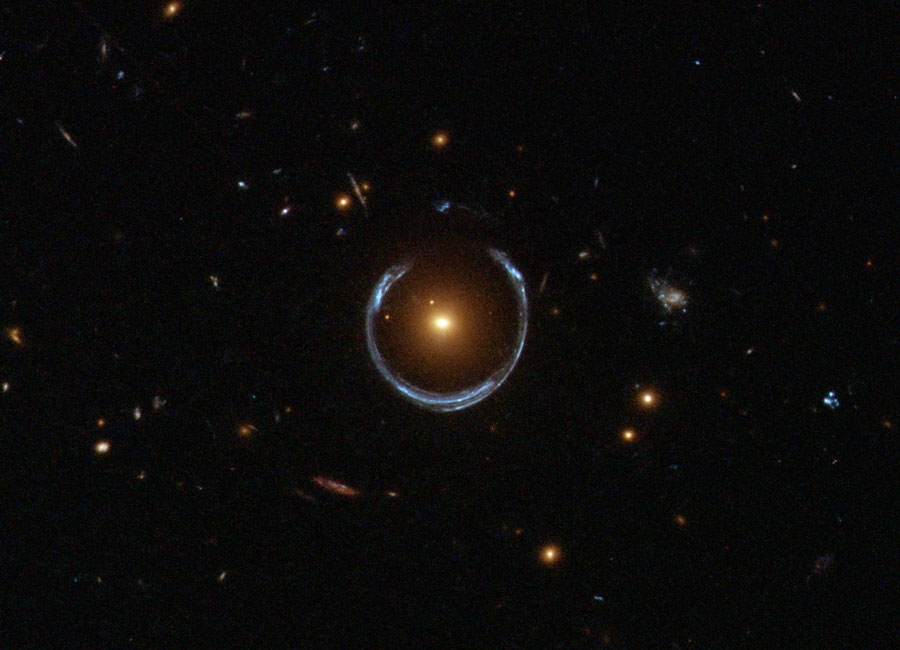
\includegraphics[width=\textwidth]{./Pictures/einstein_ring.jpg}
\caption{Image form the Hubble's Wide Field Camera 3 showing an Einstein ring. Central galaxy is the luminous red galaxy LRG-3-757. The blue annulus is a distant galaxy located behind the LRG. Image credit: NASA.}
\label{fig:einstein_ring}
\end{center}
\end{figure}
\newline

Finding Einstein rings may be a product of serendipity or digging hard on wide-field images \cite{2017arXiv170402744J}. Nevertheless, the probability of finding a system where observer-lens-source are aligned is very remote and only a small number of Einstein rings are known ($\sim20$ on the Dark Energy Survey Science Verification data). A general solution, where the system is not aligned can be found with the gravitational lens equation.

\section{Lens Equation on Gravitational Fields}
Since all the photons emitted by the source are bended coherently by the lens, the axis observer-lens constitute an optical convergent system. Thus a lens equation can be deduced using Geometrical Optics with the deflection angle ($\hat\alpha$) of a light ray --photon trajectory-- given by General Relativity \cite{Weinberg,2001PhR...340..291B,2006glsw.conf.....M,2008ARNPS..58...99H,2041-8205-723-1-L13,Weinberg201387,2015RPPh...78h6901K}:
\begin{equation}
\hat\alpha = \frac{4G_NM}{\xi c^2}.
\label{eq:deflection_angle}
\end{equation}
Here $M$ is the mass of the point-particle (lens hereafter), $G_N$ is Newton's constant, $c$ the speed of light and $\xi$ the closest encounter distance (a.k.a. impact paramenter). Using \autoref{fig:optical_system} as reference and defining $\theta$ as the observed and $\beta$ the real lens-source angle, it can be deduced that
\begin{equation}
\beta = \theta - \frac{D_{ds}}{D_s}\hat\alpha(D_d\theta)=\theta-\alpha(\theta),
\label{eq:lens_equation}
\end{equation}
where $D_{ds},D_s$ and $D_d$ are the source-lens, observer-source and observer-lens comoving distances.
\begin{figure}
\begin{center}
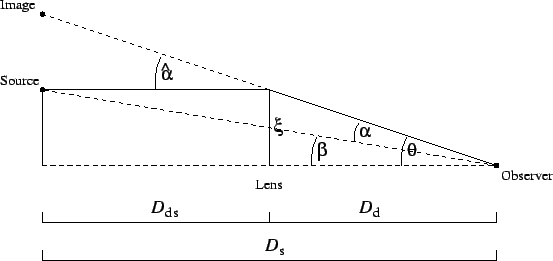
\includegraphics[width=0.9\textwidth]{optical_system.png}
\caption{Optical system of the gravitational lensing caused by a point mass. Solid line is the actual photon trajectory. Dashed lines are the apparent trajectories with and without lensing. The distances $D_s,D_d,D_{ds}$ are expressed in comoving coordinates. }
\label{fig:optical_system}
\vspace{1cm}
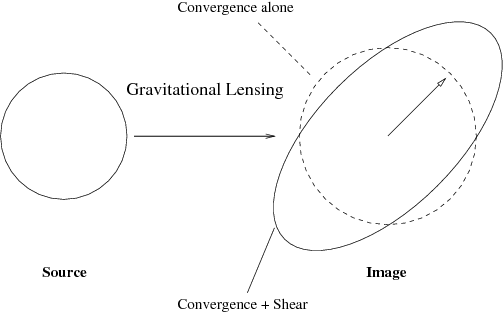
\includegraphics[width=0.9\textwidth]{./Pictures/distortion.png}
\caption{Weak-lensing distortion of an extended spherical object. Convergence leads to an isotropic enlargement, whereas shear produces an elongation/shrink along one axis.}
\label{fig:wl_distortion}
\end{center}
\end{figure}
\newline

Considering now an extended matter distribution, with density $\rho(\vec r)$, where the observer is located at the origin. The position vector can be splitted such that
\begin{equation}
\vec r = r_\parallel \hat r_\parallel + \vec r_\perp,
\end{equation}
where $r_\parallel\hat r_\parallel$ denotes the position on the direction defined by the axis observer-lens (line-of-sight or LoS hereafter) and $\vec r_\perp$ denotes a 2D vector on the plane transverse to the line-of-sight. Thus, the total matter distribution that the photon goes trough from the source to the observer is given by
\begin{equation}
\Sigma(\vec r_\perp,r_\parallel^S) = \int\limits_0^{r_\parallel^S} dr_\parallel\rho(r_\parallel,\vec r_\perp),
\label{eq:surface_density}
\end{equation}
where $\vec r^S$ is the position of the source and the quantity $\Sigma$ is called the surface density. Taking into account the flat-sky approximation --that is, all the transverse planes to LoS are parallel-- and summing to all the lens positions, \autoref{eq:deflection_angle} becomes
\begin{equation}
\hat\vec\alpha(\vec r_\perp,r_\parallel^S) = \frac{4G_N}{c^2}\int d^2\vec r_\perp \Sigma(\vec r_\perp,r_\parallel^S)\frac{\vec r^S_\perp-\vec r_\perp}{|\vec r^S_\perp-\vec r_\perp|^2}.
\end{equation}
This leads to a deflection angle
\begin{equation}
\hat \vec\alpha(\vec r_\perp,r_\parallel^S) = \frac1{\pi}\int d^2\vec r_\perp\kappa(\vec r_\perp,r_\parallel^S)\frac{\vec r^S_\perp-\vec r_\perp}{|\vec r^S_\perp-\vec r_\perp|^2},
\end{equation}
where the convergence ($\kappa$) and critical density ($\Sigma_c$) has been defined such that
\begin{equation}
\kappa(\vec r_\perp,r_\parallel^S) = \frac{\Sigma(\vec r_\perp,r_\parallel^S)}{\Sigma_c} \mbox{ with } \Sigma_c = \frac{c^2}{4\pi G_N}\frac{D_s}{D_dD_{ds}}.
\label{eq:kappa_definition}
\end{equation}
As weak-lensing wide-field surveys start to proliferate, the limit of validity of the flat-sky approximation is being reached \cite{2016arXiv161104954K,2017arXiv170205301K,2017arXiv170401054L}. Defining the lensing potential as
\begin{equation}
\psi(\vec r_\perp,r_\parallel^S) = \frac1{\pi}\int d^2\vec r_\perp\kappa(\vec r_\perp,r_\parallel^S)\ln|\vec r^S_\perp-\vec r_\perp|,
\end{equation}
the deflection angle can be written as the gradient of the lensing potential on the transverse plane
\begin{equation}
\hat\vec\alpha(\vec r_\perp,r_\parallel^S) = \nabla_\perp\psi(\vec r_\perp,r_\parallel^S)
\end{equation}
and the convergence as its laplacian,
\begin{equation}
\kappa(\vec r_\perp,r_\parallel^S)=\frac{1}{2}\nabla^2_\perp\psi(\vec r_\perp,r_\parallel^S).
\end{equation}
Thus, the lens equation from \autoref{eq:lens_equation} results
\begin{equation}
\vec\beta = \vec\theta-\nabla_\perp\psi(\vec r_\perp,r_\parallel^S).
\label{eq:lens_equation_2d}
\end{equation}
Taking into account the definition of the lensing potential, it can also be written in terms of the Newtonian gravitational potential ($\Phi$):
\begin{equation}
\psi(\vec r_\perp,r_\parallel^S) = \frac{D_{ds}}{D_sD_d}\frac{2}{c^2}\int dr_\parallel^S\Phi(D_d\vec r_\perp,r_\parallel^S).
\end{equation}
Thus, gravitational lensing is a direct probe for the underlying gravitational field.

\section{Weak Gravitational Lensing}

In addition to the change in the observed position of the source, considering no absorption nor emission of photons between the source and the observer, Liouville's theorem implies that the surface brightness of the source ($I_S$)is conserved,
\begin{equation}
I_S(\vec r_\perp) = I_S[\vec\beta(\vec r_\perp)].
\end{equation}
Considering the weak-field regime, the lensing map can be linearized such that
\begin{equation}
I_S(\vec r_\perp)=I_S[\vec\beta_0+\mathcal{J}(\vec r_{\perp 0})(\vec r_\perp-\vec r_{\perp0})],
\end{equation}
where $\mathcal{J}(\vec r_\perp)$ is the jacobian matrix. By the integration-by-substitution theorem of calculus, the integral of the surface brightness at the lensed and un-lensed coordinate systems are related by
\begin{equation}
\int I_S(\vec\beta)d\vec\beta = \det(\mathcal{J})\int I_S[\vec\beta(\vec r_\perp)]d\vec r_\perp,
\end{equation}
where $\det(\mathcal{J})$ denotes the determinant of the jacobian matrix. Thus, defining the luminosity of an extended object as the integral of its surface brightness, the luminosity for the cases with and without gravitational lensing ($L_\mu,L_0$ respectively) are related by
\begin{equation}
L_\mu = \frac{1}{\det(\mathcal{J})}L_0 = \mu L_0,
\end{equation}
where $\mu$ is called the magnification factor and is defined as de inverse of the determinant of the jacobian matrix of the lensing map.
\newline

Taking into account that the jacobian matrix is given by $\mathcal{J}=(\hat n_\perp\cdot\nabla_\perp)\vec\beta$ with $\hat n_\perp$ a unit vector on the plane transverse to LoS, by \autoref{eq:lens_equation_2d} the jacobian can be expressed as
\begin{equation}
\mathcal{J} = (\hat n_\perp\cdot\nabla_\perp)\vec r_\perp-\mathcal{J} = (\hat n_\perp\cdot\nabla_\perp)\nabla\psi,
\end{equation}
resulting finally 
\begin{equation}
\mathcal{J}(\vec r_\perp) = \left(\delta_{ij}-\frac{\partial^2\psi}{\partial r_i\partial r_j}\right)=\left( \begin{array}{c c}1-\kappa-\gamma_1 & -\gamma_2\\-\gamma_2 & 1-\kappa+\gamma_1\end{array} \right).
\label{eq:jacobian}
\end{equation}
Here $\kappa$ is the convergence, an isotropic shape distortion and $\gamma_1,\gamma_2$ is the shear, an elongation/shrink on the shape along one of the axis (\autoref{fig:wl_distortion}).
\newline

Taking into account the Born approximation --that is, the light rays of a source galaxy are deflected by only one lens--, the derivatives of the previous equation can be evaluated on the unlensed coordinates.

\subsection{Magnification}
As it has been demonstrated at the previous section, gravitational lensing increases the observed luminosity on an extended object \cite{1989Sci...245..824B,1992RvMA....5..259B,1992LNP...406..345B,1995A&A...303..643B,1995AIPC..336..307B} such that $L_\mu = \mu L_0$ with 
\begin{equation}
\mu = \frac1{(1-\kappa)^2+\gamma_1^2+\gamma_2^2}\simeq 1+2\kappa,
\label{eq:mu_definition}
\end{equation}
where on the last step it has been used that $1\gg\kappa\gg\gamma$. Taking into account the definition given at \autoref{eq:kappa_definition}, the convergence suffered by the photons emitted by a source located on the sky direction $\hat n$ and redshift $z$ is given by
\begin{equation}
\kappa(\hat n,z) = \frac{1}{2}\frac{\Sigma(\hat n,z)}{\Sigma_c}.
\end{equation}
Using the definition given at \autoref{eq:surface_density} and the poisson equation for the gravitational field this leads to
\begin{equation}
\kappa(\hat n,z) = \int\limits_0^zdz'\frac{r(z')[r(z)-r(z')]}{r(z)}\nabla_\perp\Phi(\hat n,z'),
\label{eq:kappaphi}
\end{equation}
where $r(z)$ is the comoving distance at redshift $z$ and $\Phi$ the gravitational potential. Expressing now the gravitational potential as an homogeneus therm plus a perturbation ($\Phi = \bar\Phi+\delta_\Phi$), the previous equation can be expressed as a funcion of the matter density contrast ($\delta_M$)
\begin{equation}
\nabla^2\Phi(\hat n,z) = \nabla^2\delta_\Phi(\hat n,z) = 4\pi Ga^2\bar\rho\delta_M(\hat n,z),
\label{eq:kappadeltam}
\end{equation}
where $a=1/(1+z)$ is the scale factor and $\bar\rho$ is the average density. This leads finally to \cite{PhysRevD.76.103502,PhysRevD.77.063526}
\begin{equation}
\kappa(\hat n,z) = \frac{3H_0\Omega_M(z)}{2c^2}\int\limits_0^zdz'\frac{r(z')[r(z)-r(z')]}{(1+z')r(z)}\delta_M(\hat n,z).
\label{eq:kappadeltam}
\end{equation}
The convergence, is the physical observable of Magnification and it traces the matter on the direction of line of sight whereas shear proves the matter on the transverse direction. This makes magnification and shear complementary measurements of the same phenomena. The dependence of magnification is usually splitted into two pieces: the lensing kernel,
\begin{equation}
\mathcal{K}(z) = \frac{r(z')[r(z)-r(z')]}{(1+z')r(z)}.
\end{equation}
and the matter density contrast ($\delta_M$). The lensing kernel contains only geometrical information and, for a given set of cosmological parameters, it is fixed. On the other side, the matter density contrast depends strongly on the population of galaxies selected as lens sample.
\newline

The convergence of the foreground sample can be probed tracing the three effects that it produces on the background sample:
\begin{itemize}
\item {\bf Change of the observed density:} The increase of the observed luminosity of the galaxies, allows to see sources that if there were no lensing, would be below our observational threshold nearby the location of the lenses. At the same time, an stretching of the solid angle behind the lenses causes a drop in the number density. This two effects compete between them and who is over the other depends on the slope of the number counts of the sources. Thus, at the neighbourhood of the lenses, a change of the number density respect to the average is produced. This is known as number-counts magnification.
\item {\bf Shift on the observed magnitude:} Since the increase of luminosity due to gravitational lensing is a short range effect, a shift on the observed magnitudes may be detected nearby the positions of the lenses. This requires, in principle, the knowledge of the unlensed magnitude of the sources. Nevertheless, although galaxies have a large variety of magnitudes, it can be assumed that, they are randomly distributed. Thus shifts on the magnitudes respect to the average can be detected.
\item {\bf Size enlargement:} All the effects above are a consequence that the meanwhile surface brightness is conserved, a size enlargement is produced. This effect can be statistically measured despite the fact that the unlensed size is not known. Nevertheless, since galaxies have a large variety of shape and size that is strongly related to its evolution and age, no homogeneity assumption can be made and require the definition of the {\it fundamental plane} \cite{2003AJ....125.1866B}. That kind of work is beyond the scope of this Thesis and further information can be found at Huff \& Graves 2014 \cite{2041-8205-780-2-L16}.
\end{itemize}

Traditionally all these probes have been used independently, but the ideal scenario would be a three-way combination that may lead to a cancellation or better estimation of systematic errors.
\newline

As it has been mentioned before, the knowledge of the unlensed properties of the sources is physically impossible. Thus, all the observable quantities must be formulated in terms of changes of its variation respect the ensemble average with the distance to the lenses. The statistical way to do this is the two-point angular correlation-function. This method, provides a measurement of the average convergence profile of the lenses ($\kappa(\theta)$) as a function of its angular distance $\theta$ of a point to the lens.

\subsubsection{Estimation of $\kappa(\theta)$ with the number counts technique}
The two-point angular cross-correlation between the lens ($L$) and the source ($S$) is defined as \cite{PhysRevD.77.023512,}
\begin{equation}
\omega_{LS}(\theta) = \langle\delta_O(\hat n,z_L,f_\mu)\delta_O(\hat n',z_S,f_\mu)\rangle_{\theta}.
\label{eq:2pacfmagnification}
\end{equation}
Where $\delta_O(\hat n,z_L,f_\mu)$ is the observed galaxy density-contrast on the sky direction $\hat n$ and redshift $z_L$ with flux limit $f_\mu$. Since due to magnification galaxies beyond the observable threshold will appear nearby the lenses introducing a non-uniform distribution of galaxies. Thus the observed galaxy density contrast can be expressed as
\begin{equation}
\delta_O(\hat n,z,f_\mu) = \delta_g(\hat n,z)+\delta_\mu(\hat n,z,f_\mu),
\end{equation}
where $\delta_g$ is the intrinsic galaxy-density contrast (that is, without magnification) and $\delta_\mu$ is the density contrast due to magnification. Thus \autoref{eq:2pacfmagnification} becomes
\begin{equation}
\omega_{LS}(\theta) = \langle\delta_g(z_L)\delta_g(z_S)\rangle+\langle\delta_g(z_L)\delta_\mu(z_S)\rangle+\langle\delta_\mu(z_L)\delta_g(z_S)\rangle+\langle\delta_\mu(z_L)\delta_\mu(z_S)\rangle.
\label{eq:4t}
\end{equation}
Taking into account that $0<z_L<z_S$, and that the lens and the source sample are well redshift separated, the only non vanishing term is
\begin{equation}
\omega_{LS}(\theta) = \langle\delta_g(\hat n,z_L)\delta_\mu(\hat n,z_L,f_\mu)\rangle_\theta.
\end{equation}
Let define the magnification density contrast on the sky direction $\hat n$ as 
\begin{equation}
\delta_\mu(\hat n,z,f_\mu) = \frac{N_\mu(\hat n,z,f_\mu)}{N_0(\hat n,z,f_0)}-1,
\end{equation}
where $N_0(\hat n,z,f_0)$ is the un-lensed cumulative number counts of sources located at redshift $z$, that is, the number of sources with observed flux greater than the threshold $f_0$. Conversely, $N_\mu(\hat n,z,f_\mu)$ is the lensed cumulative number counts affected by magnification.
\newline

Magnification by gravitational lenses increases the observed flux of background objects  allowing to see fainter sources by an amount $f_\mu = f_0/\mu$. At the same time, it stretches the solid angle behind the lenses, reducing the surface density of sources an amount $N_\mu = N_0/\mu$, which translates into the density contrast as:
\begin{equation}
\delta_\mu(\hat n,z,f_\mu) = \frac{N_\mu(\hat n,z,f_\mu)}{\mu N_\mu(\hat n,z,\mu f_\mu)}-1.
\label{eq:magnification_density_contrast}
\end{equation}
The cumulative number counts can be locally parametrized as a power law
\begin{equation}
N_\mu(\hat n,z,f_\mu) = A\left(\frac{f_\mu}{f_*}\right)^{\alpha(f_\mu)},
\end{equation}
where $A,f_*$ are constant parameters and $\alpha(f_\mu)$ a function of the flux limit. Substituting this into \autoref{eq:magnification_density_contrast}
\begin{equation}
\delta_\mu(\hat n,z,f_\mu) = \mu^{\alpha(f_\mu)-1}-1.
\end{equation}
Taking into account the weak-lensing approximation $\mu\simeq 1+2\kappa$ along with \autoref{eq:mu_definition} and translating from fluxes to magnitudes this results
\begin{equation}
\delta_\mu(\hat n,z,m) = 2\kappa(\hat n,z)[\alpha(m)-1]
\end{equation}
with
\begin{equation}
\alpha(m) = 2.5\frac{d}{dm}\left[\log N_\mu(m)\right].
\label{eq:alpha}
\end{equation}
Thus \autoref{eq:2pacfmagnification} becomes
\begin{equation}
\omega_{LS}(\theta) = 2[\alpha(m)-1]\langle\delta_g(\hat n,z_L)\kappa(\hat n',z_S)\rangle_\theta = [\alpha(m)-1]2\kappa(\theta),
\end{equation}
where $\kappa(\theta)$ is the convergence profile of the selected lenses.

\subsubsection{Estimation of $\kappa(\theta)$ with magnitude-shift magnification technique}
The magnitude-position-angular correlation function between the lens sample ($L$) and the source sample ($S$) is defined as
\begin{equation}
\varphi_{LS}(\theta) = \langle\delta_g(z_L,\hat n)\delta_m(z_S,\hat n')\rangle_\theta.
\label{eq:mpacf}
\end{equation}
Where, as on  the last section $\delta_g (z,\hat n)$ is the galaxy density contrast at redshift $z$ on the sky direction $\hat n$ and $\delta_m$ is the magnitude shift\footnote{Do not confuse with $\delta_M$, the matter density contrast.}, defined as
\begin{equation}
\delta_m(z,\hat n) = m_\mu(\hat n,z)-m_0(\hat n,z),
\end{equation}
where $m_\mu$ is the lensed magnitude and $m_0$ the unlensed magnitude. Taking into account that, as it has been demonstrated previously
\begin{equation}
f_\mu(\hat n,z) = \mu(\hat n,z)f_0(\hat n,z) \Leftrightarrow m_\mu(\hat n,z)-m_0(\hat n,z) = -2.5\log\mu(\hat n,z),
\end{equation}
where on the last step it has been converted from fluxes to magnitudes. Thus, taking into account that
\begin{equation}
\log(\mu) \simeq \log(1+2\kappa)\simeq 2\kappa,
\end{equation}
the \autoref{eq:mpacf} results finally
\begin{equation}
\varphi_{LS}(\theta)= -5\langle\delta_g(\hat n,z_L)\kappa(\hat n',z_S)\rangle = -5\kappa(\theta),
\end{equation}
where $\kappa(\theta)$ is the convergence profile of the lenses.
\newline

Nevertheless, reddening by the inter-galactic medium  can also produce --unlike gravitational lensing-- wavelength-dependent magnitude-shifts. Thus, the lensed-plus-reddened fluxes are given by
\begin{equation}
f_\mu(\hat n,z,\lambda_\eta) = \mu(\hat n,z)f_0(\hat n,z)e^{-\tau(\lambda_\eta)},
\end{equation}
that converted to magnitudes results in
\begin{equation}
m_\mu(\hat n',z,\lambda_\eta)-m_0(\hat n',z,\lambda_\eta)=-2.5\log\mu+\frac{2.5}{\ln 10}\tau(\lambda_\eta),
\end{equation}
where $\tau(\lambda_\eta)$ is the optical depth at the wavelength $\lambda_\eta$. The dust and the lensing components can be disentangled by defining the color-excess angular correlation function ($E^{\eta\nu}$) between two-wavelengths $\lambda_\eta,\lambda_\nu$,
\begin{equation}
E^{\eta\nu}_{LS}(\theta) = \langle\delta_g(\hat n,z_L)[m_\mu(\hat n',z_S,\lambda_\eta)-m_\mu(\hat n',z_S,\lambda_\nu)]\rangle_\theta.
\end{equation}
Since gravitational lensing is acromatic, the only dependence with the wavelength comes from the extinction law
\begin{equation}
E^{\eta\nu}_{LS}(\theta)=\frac{2.5}{\ln 10}\langle\delta_g(\hat n,z_L)[\tau(\hat n',z_S,\lambda_\eta)-\tau(\hat n',z_S,\lambda_nu)]\rangle.
\end{equation}

Modeling the wavelength dependence of the optical depth as
\begin{equation}
\tau_\eta = \tau(\lambda_\eta) = \tau_V\left(\frac{\lambda_V}{\lambda_\eta}\right)^\gamma,
\end{equation}
where $\tau_V$ is the optical depth at the $V$-band filter, $\lambda_V$ is the wavelength of the $V$-band filter and $\gamma\sim 1$ is a constant parameter. Thus, the color-excess cross-correlation results finally
\begin{equation}
E^{\eta\nu}_{LS}(\theta)=\lambda_V(\lambda_\eta^{-1}-\lambda_\nu^{-1})\frac{2.5}{\ln 10}\langle\delta_g(\hat n,z_L)\tau_V(\hat n',z_S)\rangle.
\end{equation}
At a wide field survey with several broad-band band-pass filters the scale dependence of the optical depth, $\tau_V(\hat n,z_S)$ can be constrained.

\subsection{Shear}
From the Jacobian of the lensing map, it can be deduced that the transformation is not isotropic producing an elongation along one of the axis $(r_1,r_2) = \vec r_\perp$. Thus, an intrinsically round galaxy is seen as elliptical. On the case of elliptical galaxies, statistically they present a global ellipticicity. From the definition of \autoref{eq:jacobian}, the shear components are given by:
\begin{equation}
\gamma_1(\vec r_\perp) = -\frac{1}{2}\left(\frac{\partial^2\psi}{\partial r_1^2}-\frac{\partial^2\psi}{\partial r_2^2}\right)\mbox{ and }\gamma_1(\vec r_\perp) = -\frac{\partial^2\psi}{\partial r_1\partial r_2}.
\end{equation}
The shear fields $\gamma_1,\gamma_2$ can be expressed as Fourier series such that:
\begin{equation}
\tilde \gamma_{1,2}(\vec k_\perp) = \int \gamma_{1,2}(\vec r_\perp)e^{-i\vec k_\perp\cdot\vec r_\perp}d^2\vec r_\perp
\end{equation}
and
\begin{equation}
\gamma_{1,2}(\vec r_\perp) = \frac{1}{(2\pi)^2}\int \tilde\gamma_{1,2}(\vec k_\perp)e^{i\vec k_\perp\cdot\vec r_\perp}d^2\vec k_\perp.
\end{equation}
Expressing the differential equation at the Fourier space with the usual approach $\partial/\partial r_1\rightarrow ir_1$ it leads to
\begin{equation}
\gamma_1(\vec k_\perp) = \frac{1}{2}(r_1^2-r_2^2)\tilde\psi(\vec k_\perp)\mbox{ and }\gamma_2(\vec k_\perp) = \frac{1}{2}r_1r_2\vec \psi(\vec r_\perp)
\end{equation}

Considering a plane-wave perturbation of the lensing potential, it is useful to align the axis of the perturbation with those of the shear field such that
\begin{equation}
\tilde \gamma_E(\vec k_\perp) = \cos(2\phi_{\vec k_\perp})\tilde \gamma_1(\vec k_\perp)+\sin(2\phi_{\vec k_\perp})\tilde \gamma_2(\vec k_\perp)
\end{equation}
and
\begin{equation}
\tilde \gamma_B(\vec k_\perp) = \cos(2\phi_{\vec k_\perp})\tilde \gamma_1(\vec k_\perp)-\sin(2\phi_{\vec k_\perp})\tilde \gamma_2(\vec k_\perp).
\end{equation}
Resulting finally that
\begin{equation}
\tilde\gamma_E(\vec k_\perp) = \vec k_\perp^2\tilde\psi(\vec k_\perp)\mbox{ and }\tilde\gamma_B(\tilde k_\perp) = 0
\end{equation}
The fact that $\gamma_B$ is zero, constitutes a necessary (but not sufficient) proof for the lack of systematic effects on any shear measurement.
\newline

Reaching this point, two kinds of two-point statistics can be build: the point-shear\footnote{This is usually called galaxy-galaxy- (or gg-) lensing.} and the shear-shear two-point angular-correlation functions. From this two, we will only focus to gg-lensing due to its direct connection to magnification.

\subsubsection{The gg-lensing.}
Defining $\tilde\epsilon$ as the observed ellipticity, taking into account shear distortions it can be expressed as:
\begin{equation}
\tilde\epsilon = \tilde\epsilon_i + \tilde\gamma,
\end{equation}
where $\tilde\epsilon_i$ is the intrinsic ellipticity of the galaxy. As stated previously, without loss of generality, shear coordinates can be rotated.  Thus, let define the tangential shear $\gamma_t$ as
\begin{equation}
\gamma_t = -[\cos(2\phi_{\vec k_\perp})\tilde \gamma_1(\vec k_\perp)+\sin(2\phi_{\vec k_\perp})]\tilde \gamma_2(\vec k_\perp) = -\gamma_E.
\end{equation}
On the new coordinates, this leads to
\begin{equation}
\epsilon = \epsilon_i+\gamma_E,
\end{equation}
where $\tilde\epsilon,\tilde\epsilon_i$ are the ellipticity on the new coordinates. Let $p(\epsilon)$ the distribution of ellipticity of the sources.  At the small distortion regime, assuming that ellipticity is isotropic, it follows that
\begin{equation}
p(\epsilon) = p(\epsilon_i)+\gamma_t\cos2\phi\frac{\partial p(\epsilon)}{\partial \epsilon}.
\end{equation}
Here $\phi_{\vec k_\perp}$ is the angle of orientation of the principal axis of the galaxy. Integrating over all the ellipticity, they can be translated to orientation angle,
\begin{equation}
p(\phi) = \frac{2}{\pi}\left[1-\langle\gamma_t\rangle\cos2\phi\left\langle\frac1{\epsilon}\right\rangle\right].
\end{equation}
Thus, measuring the ellipticity --or orientation angles--, shear E-modes can be measured, probing directly the underlying lensing potential.
\newline

Tangential shear can be estimated to be
\begin{equation}
\langle\gamma_t\rangle = -\frac{\Delta\Sigma}{\Sigma_c},
\end{equation}
with
\begin{equation}
\Delta\Sigma = \bar\Sigma(\theta)-\Sigma(\theta),
\end{equation}
where $\bar\Sigma(\theta)$ denotes the average surface density on an disk of angular size $\theta$. Thus the tangential shear can be related to the convergence profile as
\begin{equation}
\langle\gamma_t\rangle=-[\bar\kappa(\theta)-\kappa(\theta)].
\end{equation}
\newline

The last equation demonstrates that gg-lensing and magnification are produced by the same physical effect. Nevertheless, they have different systematic effects. This can be exploited in order to produce accurate and reliable magnification measurements. 

\section{Theoretical expressions for $\kappa(\theta)$}
As it has been stated on the previous section, the convergence profile  is the physical observable for both magnification and gg-lensing. Thus, in order to connect the measurements with a cosmological model, a theoretical expression for it must be provided. Depending on the nature of the lenses considered --that is, whether the lenses are galaxies, voids, clusters or troughs--, the approach may differ.
\newline

On this section, are only provided the solutions for galaxies and voids. Although troughs will also be considered on the data analysis, it is beyond the scope of this Thesis and it is still part of an ongoing project. A simple solution can be found on Gruen et~al. \cite{2016MNRAS.455.3367G}. Nevertheless, a more general and complete solution is still to be published.
\newline

The simplest solution for the convergence profile, is for a sample of galaxies. Taking into account the definition of $\kappa$
\begin{equation}
\kappa(\theta) = \langle\delta_g(\hat n,z_L)\kappa(\hat n',z_S)\rangle_\theta,
\end{equation}
if a linear, constant and redshift-independent galaxy-bias ($b_L$) is considered; a relation between the galaxy density contrast $\delta_g$ and matter density contrast $\delta_M$ can be established:
\begin{equation}
\delta_g(\hat n,z_L) = b_L\delta_M(\hat n,z_L).
\end{equation}
Thus, the convergence profile is given by
\begin{equation}
\kappa(\theta) = b_L\langle\delta_M(\hat n,z_L)\kappa(\hat n',z_S)\rangle_\theta.
\end{equation}
If it is considered that the convergence field $\kappa(\hat n)$ can be expressed also as a function of the matter density contrast by \autoref{eq:kappadeltam} and \autoref{eq:kappaphi}:
\begin{equation}
\kappa(\theta) = b_L\left\langle\delta_M(\hat n,z_L)\left[\int\limits_0^zdz'\frac{r(z')[r(z)-r(z')]}{r(z)}4\pi Ga^2\bar\rho\delta_M(\hat n,z)\right]\right\rangle.
\end{equation}
This leads finally to \cite{2003A&A...403..817M}:
\begin{eqnarray}
&\kappa(\theta)=\frac{3H_0^2\Omega_M^0}{c^2}\int\limits_0^\infty dz'_L\frac{\phi_L(z'_L)}{1+z'_L}\int\limits_{z'_L}^\infty dz'_S\phi_S(z'_S)\frac{r(z'_L)[r(z'_S)-r(z'_L)]}{r(z'_S)}\times\\
&\int\limits_0^\infty\frac{dkk}{2\pi}P_M(k,z'_L)J_0[k\theta r(z'_i)],\nonumber
\label{eq:omega0}
\end{eqnarray}
where $\phi_L,\phi_S$ are the redshift distributions of the lens and source sample respectively, $P_M$ the matter power spectrum of the lens sample and $J_0$ is the zero-th order Bessel function.
\newline

The calculation of the convergence profile for a void needs to assume a void profile. A general LTB solution on General Relativity for voids can be found at \cite{2008JCAP...04..003G,2016MNRAS.455.1246F,2016MNRAS.462.1882K}, 
\begin{equation}
\delta(r_v) = \delta_0g(a)\left(1-\frac{2}{3}\frac{r_v^2}{r_0^2}\right)\exp\left(-\frac{r_v^2}{r_0^2}\right),
\end{equation}
where $r_v$ is the radial comoving distance {\bf on the system of coordinates centered at the void}, $r_0$ the radial size of the void, $\delta_0$ the central underdensity and $g(a)$ the growth factor {\bf not normalized at present}. On the system of coordinates centered on the observer and considering non-spherical voids, this leads to the Kovacs \& Garcia-Bellido void-profile (KGB):
\begin{equation}
\delta_{KGB}(\theta,z) = \delta_0g(a)\left[1-\frac{2}{1+2q^2}\left(\frac{r_\parallel^2}{r_0^2}+\frac{q^2r_\perp^2}{r_0^2}\right)\right]\exp\left[-\left(\frac{r_\parallel^2}{q^2r_0^2}+\frac{r_\perp^2}{r_0^2}\right)\right],
\label{eq:kgb}
\end{equation}
where $q^2=1-e^2$ with $e$ the ellipticity of the void and
\begin{eqnarray}
&r_\parallel=r(z)\cos\theta -r(z_v)\\
&r_\perp=r(z)\sin\theta.
\end{eqnarray}
Here $r(z)$ is the radial comoving distance at redshift $z$, whereas $z_v$ is the redshit of the center of the void and $\theta$ the angular separation form the center of the void. From \autoref{eq:kgb} and \autoref{eq:kappa_definition}, the convergence profile around a single void can be obtained:
\begin{equation}
\kappa(\theta) = \frac{1}{1}\frac{\Sigma_{KGB}(\theta)}{\Sigma_c},
\end{equation}
where the surface density is given by
\begin{equation}
\Sigma_{KGB}(\theta) = \int\limits_0^\infty dz'\bar\rho_M(z')[\delta_{KGB}(\theta,z')-1].
\end{equation}
Here the $\bar\rho_M(z')$ is the matter average density of the Universe at redshift $z'$, given by
\begin{equation}
\bar\rho(z') = \frac{\Omega_M^0\rho_c}{(1+z')^3}
\end{equation}
with $\rho_c$ the critical energy density of the Universe.